\id{МРНТИ 28.17.19}{}

\begin{articleheader}
\sectionwithauthors{М.С. Әлиаскар, Ш.А. Джомартова, Ә.Т. Мазақова, Т.Ж. Мазақов, А.Д. Майлыбаева, Н.Т. Исимов, К.Б. Бегалиева, А.Т. Досаналиева}{ПРИМЕНЕНИЕ ЧИРПЛЕТОВ ДЛЯ ИДЕНТИФИКАЦИИ ЧЕЛОВЕКА ПО АУДИОЗАПИСЯМ}

{\bfseries
\textsuperscript{1,2}М.С. Әлиаскар,
\textsuperscript{2}Ш.А. Джомартова\textsuperscript{\envelope },
\textsuperscript{2}Ә.Т.Мазақова,
\textsuperscript{1,2}Т.Ж. Мазақов,
\textsuperscript{3}А.Д. Майлыбаева,
\textsuperscript{1}Н.Т. Исимов,
\textsuperscript{4}К.Б. Бегалиева,
\textsuperscript{5}А.Т. Досаналиева
}
\end{articleheader}

\begin{affiliation}
\textsuperscript{1}Международный инженерно-технологический университет, Алматы, Казахстан,

\textsuperscript{2}Казахский национальный университет им. аль-Фараби, Алматы, Казахстан,

\textsuperscript{3}Атырауский университет им. Х. Досмухамедова, Атырау, Казахстан,

\textsuperscript{4}Казахский агротехнический исследовательский университет им. С. Сейфуллина, Астана, Казахстан,

\textsuperscript{5}Алматинский Технологический Университет, Алматы, Казахстан

\raggedright \textsuperscript{\envelope } Корреспондент-автор: \href{mailto:jomartova@mail.ru}{jomartova@mail.ru}
\end{affiliation}

Статья посвящена решению ряда задач, возникающих при изучении
аудиосигналов. Предложенный алгоритм реализован на Python и применен для
анализа аудиозаписей. Эффективность предлагаемого авторами алгоритма
демонстрируется при обработке речевой информации для выделения
характеристик голоса конкретного человека.

Разработанный алгоритм основан на применении чирплетов к обработке
звуковых сигналов, отличается универсальностью и возможностями быстрой
адаптации к различным приложениям. В статье представлены результаты
численных расчетов и оценены дальнейшие перспективы развития подобных
систем.

Представленные в работе алгоритмы могут быть применены при обработке
сигналов различной природы физических, химических и экономических
процессов.

{\bfseries Ключевые слова:} интеллектуальная система, преобразования Фурье,
очистка сигнала, распознавание голоса, чирплет.

\begin{articleheader}
{\bfseries АУДИО ЖАЗБАЛАРДАН АДАМДАРДЫ АНЫҚТАУ ҮШІН CHIRPLETS ПАЙДАЛАНУ}

{\bfseries
\textsuperscript{1,2}М.С. Әлиаскар,
\textsuperscript{2}Ш.А. Джомартова\textsuperscript{\envelope },
\textsuperscript{2}Ә.Т.Мазақова,
\textsuperscript{1,2}Т.Ж. Мазақов,
\textsuperscript{3}А.Д. Майлыбаева,
\textsuperscript{1}Н.Т. Исимов,
\textsuperscript{4}К.Б. Бегалиева,
\textsuperscript{5}А.Т. Досаналиева
}
\end{articleheader}

\begin{affiliation}
\textsuperscript{1}Халықаралық инженерлік және технология университеті, Алматы, Қазақстан,

\textsuperscript{2}Әл-Фараби атындағы Қазақ ұлттық университеті, Алматы, Қазақстан

\textsuperscript{3}Х.Досмұхамедов атындағы Атырау университеті, Атырау, Қазақстан,

\textsuperscript{4}Сейфуллин атындағы Қазақ агротехникалық зерттеу университеті, Астана, Қазақстан,

\textsuperscript{5}Алматы технологиялық университеті, Алматы, Қазақстан,

e-mail: \href{mailto:jomartova@mail.ru}{jomartova@mail.ru}
\end{affiliation}

Мақала дыбыстық сигналдарды зерттеу кезінде туындайтын бірқатар
мәселелерді шешуге арналған. Ұсынылған алгоритм Python-да енгізілген
және аудио жазбаларды талдау үшін қолданылады. Авторлар ұсынған
алгоритмнің тиімділігі белгілі бір адамның дауысының сипаттамаларын
анықтау үшін сөйлеу ақпаратын өңдеуде көрсетіледі.

Әзірленген алгоритм дыбыстық сигналдарды өңдеуге чирплеттерді қолдануға
негізделген, оның әмбебаптығымен және әртүрлі қосымшаларға тез бейімделу
мүмкіндігімен ерекшеленеді. Мақалада сандық есептеулердің нәтижелері
берілген және мұндай жүйелердің одан әрі даму перспективалары
бағаланады.

Жұмыста ұсынылған алгоритмдер физикалық, химиялық және экономикалық
процестердің әртүрлі сипаттағы сигналдарды өңдеуде қолданылуы мүмкін.

{\bfseries Түйінді сөздер:} интеллектуалды жүйе, Фурье түрлендірулері,
сигналды тазалау, дауысты тану, шырылдау.

\begin{articleheader}
{\bfseries USING CHIRPLETS TO IDENTIFY PEOPLE FROM AUDIO RECORDINGS}

{\bfseries
\textsuperscript{1,2}M.S. Aliaskar,
\textsuperscript{2}Sh.A.Jomartova\textsuperscript{\envelope },
\textsuperscript{2}A.T. Mazakova,
\textsuperscript{1,2}Т.Zh. Mazakov,
\textsuperscript{3}A.D. Mailybayeva,
\textsuperscript{1}N.T. Isimov,
\textsuperscript{4}K.B. Begaliyeva,
\textsuperscript{5}A.T. Dossanalyieva
}
\end{articleheader}

\begin{affiliation}
\textsuperscript{1}International Engineering and Technology University, Almaty, Kazakhstan,

\textsuperscript{2}Kazakh National University named after Al-Farabi, Almaty, Kazakhstan,

\textsuperscript{3}Atyrau University named after Kh. Dosmukhambetov, Atyrau, Kazakhstan,

\textsuperscript{4}Kazakh Agrotechnical Research University named after S. Seifullin, Astana, Kazakhstan,

\textsuperscript{5}Almaty Technological University, Almaty, Kazakhstan,

e-mail: \href{mailto:jomartova@mail.ru}{jomartova@mail.ru}
\end{affiliation}

The article is devoted to solving a number of problems that arise when
studying audio signals. The proposed algorithm is implemented in Python
and applied to analyze audio recordings. The efficiency of the algorithm
proposed by the authors is demonstrated when processing speech
information to identify the characteristics of a specific
person' s voice.

The developed algorithm is based on the use of chirplets to process
audio signals, is universal and can be quickly adapted to various
applications. The article presents the results of numerical calculations
and assesses the further prospects for the development of such systems.

The algorithms presented in the work can be used to process signals of
various natures of physical, chemical and economic processes.

{\bfseries Keywords:} intelligent system, Fourier transforms, signal
cleaning, voice recognition, chirplet.

\begin{multicols}{2}
{\bfseries Введение.} Технологии анализа и обработки аудиосигналов в
последние годы приобретают всё большую актуальность в связи с ростом
количества задач, связанных с распознаванием речи и биометрической
идентификацией человека по голосу. Одной из ключевых проблем в этой
области является необходимость надёжного и точного выделения
информативных признаков речи, позволяющих отличить одного говорящего от
другого. Классические спектральные методы не всегда обеспечивают должную
точность при работе с нестационарными сигналами и шумами, особенно когда
частота в сигнале меняется во времени.

В связи с этим особый интерес представляют современные методы обработки,
основанные на чирплет-преобразованиях (Chirplet Transform). Они сочетают
преимущества вейвлет-анализа и возможностей по отслеживанию изменений
частоты, позволяя более гибко анализировать сложные нестационарные
структуры. Применение чирплет-преобразования эффективно при изучении
речевых сигналов, где частота может варьироваться под влиянием
особенностей речи, интонации и акцента. Кроме того, данный подход
демонстрирует высокую универсальность и может использоваться в анализе
различных типов данных -- от радиолокационных до биомедицинских
{[}1-3{]}.

Целью данной работы является демонстрация алгоритма, реализованного на
языке Python и предназначенного для выделения ключевых частотных и
амплитудных характеристик речи. С помощью предлагаемых автором методов
можно строить системы распознавания голоса, способные автоматически
идентифицировать человека по кратким речевым фрагментам. Подход,
основанный на чирплет-преобразованиях, даёт перспективы для
масштабирования и адаптации: его можно применять при исследовании
широкого спектра сигналов, включая экономические, химические и
биомедицинские временные ряды.

В статье представлены результаты численных экспериментов, выполненных на
речевых записях нескольких десятков дикторов. Проведённый анализ
показывает, что чирплет-преобразования могут повысить точность
идентификации по сравнению с традиционными методами спектрального
анализа, особенно при наличии шума и непредсказуемых изменений в
голосовых данных. Рассматриваются основные теоретические аспекты,
описываются особенности реализации алгоритма в Python и обсуждаются
возможности дальнейшего развития данной методики.

Чирплет-преобразование является мощным инструментом для анализа
аудиосигналов, особенно в случаях, когда частота изменяется во времени.
Оно находит применение в обработке речи, музыкальном анализе, эхолокации
и биомедицинских приложениях.

{\bfseries Материалы и методы.} В рамках данной работы в качестве исходных
данных использовались аудиозаписи речи в формате WAV. Каждая запись
представляла собой последовательность чисел от одного до десяти,
произнесённых на русском языке. Всего было сформировано 50 таких файлов
от студентов Международного инженерно-технологического университета (г.
Алматы). Эксперименты также включали проверку аудио другого человека, не
входившего в базу данных, для оценки возможности выявления «чужого»
диктора.

Алгоритм обработки записей реализован на языке Python и состоит из
нескольких основных шагов:

\emph{1. Очистка сигнала от шума.}

Сначала на основе быстрого преобразования Фурье (FFT) оценивается спектр
исходного сигнала и задаётся амплитудный порог, позволяющий удалить
паразитные компоненты. Затем выполняется обратное преобразование Фурье,
в результате чего получается очищенный аудиосигнал.

\emph{2. Формирование чирплет-базиса.}

Для дальнейшего анализа строится набор (базис) чирплет-функций с разными
параметрами масштабирования (\emph{a}), временного сдвига (\emph{b}) и
коэффициента чирпа (\emph{k}). Базисные функции представляют собой
модифицированные вейвлеты, позволяющие учесть изменения частоты во
времени.

\emph{3. Вычисление коэффициентов чирплет-преобразования.}

Исходный сигнал проецируется (разлагается) на каждую из чирплет-функций.
В результате получают набор комплексных коэффициентов, отражающих вклад
соответствующих чирплет-компонент в структуру анализируемого сигнала.

4. Анализ амплитудно-частотных характеристик.

Расчётные коэффициенты разделяются на амплитудную и частотную
составляющие. Частотные значения сортируются по убыванию амплитуды,
после чего выбирается несколько наиболее значимых гармоник (в работе
использовалось \emph{Ka}=3). На этом этапе формируется набор
характеристик голоса, специфичных для конкретного человека (основные
тоны и соответствующие амплитуды).

\emph{4. Выделение и сохранение признаков.}

Отобранные амплитудно-частотные пары сохраняются в виде вектора
признаков (частотные коэффициенты и их амплитуды). Такой вектор далее
можно использовать для сравнения разных образцов речи: при небольшом
расстоянии между векторами аудиозаписи считаются принадлежащими одному
диктору; если расстояние превышает некоторый порог, дикторы полагаются
разными.

Описание результатов расчётов и графические иллюстрации (очищенного
сигнала, чирплетных разложений, амплитудных и фазовых спектров) получены
с помощью программы на Python, которая читает входные данные (WAV-файл),
выполняет указанные этапы преобразования и сохраняет итоговые величины в
текстовом файле. Систематическая проверка метода проведена на 50
записях, при этом точность автоматического распознавания дикторов
составила порядка 73--75\%. Для аудиозаписи, не содержащейся в базе
данных, метод показал способность отличать её от имеющихся образцов, что
подтверждает перспективность описанного подхода для дальнейшего развития
систем биометрической идентификации {[}4-7{]}.

Применение чирплет-анализа также представляется перспективным
направлением.

\emph{{\bfseries Теоретическая часть.}} Чирплет-преобразование (Chirplet
Transform) представляет собой обобщение вейвлет-преобразования,
учитывающее возможность изменения частоты анализируемого сигнала во
времени.

Существуют различные типы чирплетов:


1. Гауссовый чирплет (Gaussian Chirplet) - основан на гауссовых
вейвлетах;

1. Фурье-чирплет (Fourier Chirplet) - базируется на преобразованиях
Фурье;

1. Вейвлет-чирплет (Wavelet Chirplet) -- модифицирует классическое
вейвлет-преобразование, добавляя компоненту изменяющейся частоты.
Основные преимущества чирплет-преобразования:


- Адаптивность к изменяющимся частотам: даёт возможность анализировать
сигналы со сложной временной и частотной структурой.

- Комбинированная локализация во времени и частоте: позволяет точно
выделять особенности сигнала, распределённые по шкале времени и
частоты.

- Универсальность: может применяться в задачах обработки акустических,
радиолокационных и биомедицинских сигналов {[}8-10{]}.
Чирп-сигнал можно описать следующим образом:
\end{multicols}

%% \begin{longtable}[]{@{}
%%   >{\raggedright\arraybackslash}p{(\linewidth - 2\tabcolsep) * \real{0.9463}}
%%   >{\raggedright\arraybackslash}p{(\linewidth - 2\tabcolsep) * \real{0.0537}}@{}}
%% \toprule\noalign{}
%% \begin{minipage}[b]{\linewidth}\centering
%% 
%% \end{minipage} & \begin{minipage}[b]{\linewidth}\centering
%% (1)
%% \end{minipage} \\
%% \midrule\noalign{}
%% \endhead
%% \bottomrule\noalign{}
%% \endlastfoot
%% \end{longtable}

где: \emph{A} -- амплитуда,
--
начальная частота, \emph{k} -- коэффициент изменения частоты во времени
(чирп), \emph{j} -- мнимая единица
().

Базисные функции чирплет-преобразования записываются как:

%% \begin{longtable}[]{@{}
%%   >{\raggedright\arraybackslash}p{(\linewidth - 2\tabcolsep) * \real{0.9470}}
%%   >{\raggedright\arraybackslash}p{(\linewidth - 2\tabcolsep) * \real{0.0530}}@{}}
%% \toprule\noalign{}
%% \begin{minipage}[b]{\linewidth}\centering
%% 
%% \end{minipage} & \begin{minipage}[b]{\linewidth}\centering
%% (2)
%% \end{minipage} \\
%% \midrule\noalign{}
%% \endhead
%% \bottomrule\noalign{}
%% \endlastfoot
%% \end{longtable}

где:

- 
-- базовая вейвлет-функция,

- 
-- фазовый множитель, который модулирует вейвлет, добавляя эффект
чирпа.
Чирплет-преобразование позволяет разложить сигнал в базис, состоящий из
чирповых сигналов разной частоты и частотного наклона.

Базисные функции в чирплет-преобразовании представляют собой растянутые,
сдвинутые и искривленные версии исходного вейвлета.

Рассмотрим некоторую последовательность

измерений
.

Чирплет-преобразование можно вычислять дискретно для сигнала
\emph{s}{[}\emph{i}{]} следующим образом:

%% \begin{longtable}[]{@{}
%%   >{\raggedright\arraybackslash}p{(\linewidth - 2\tabcolsep) * \real{0.9463}}
%%   >{\raggedright\arraybackslash}p{(\linewidth - 2\tabcolsep) * \real{0.0537}}@{}}
%% \toprule\noalign{}
%% \begin{minipage}[b]{\linewidth}\centering
%% 
%% \end{minipage} & \begin{minipage}[b]{\linewidth}\centering
%% (3)
%% \end{minipage} \\
%% \midrule\noalign{}
%% \endhead
%% \bottomrule\noalign{}
%% \endlastfoot
%% \end{longtable}

где:


- \emph{N} -- длина сигнала,

- 
-- дискретные отсчёты сигнала,

- 
-- дискретная чирплет-функция

- \emph{a} -- масштабный параметр,

- \emph{b} -- временной сдвиг,

- \emph{k} -- параметр чирпа,

- * -- обозначает комплексное сопряжение.
В дискретном случае чирплет-функция может быть представлена как:

%% \begin{longtable}[]{@{}
%%   >{\raggedright\arraybackslash}p{(\linewidth - 2\tabcolsep) * \real{0.9470}}
%%   >{\raggedright\arraybackslash}p{(\linewidth - 2\tabcolsep) * \real{0.0530}}@{}}
%% \toprule\noalign{}
%% \begin{minipage}[b]{\linewidth}\centering
%% 
%% \end{minipage} & \begin{minipage}[b]{\linewidth}\centering
%% (4)
%% \end{minipage} \\
%% \midrule\noalign{}
%% \endhead
%% \bottomrule\noalign{}
%% \endlastfoot
%% \end{longtable}

\begin{multicols}{2}
Алгоритм реализации чиплет-обработки исходного сигнала.

Шаг 1. Пусть дана последовательность

измерений
.

Выполняется фильтрация шума на основе быстрого преобразования Фурье
(FFT). Для этого определяется амплитудный порог для удаления шума. Далее
применяется обратное преобразование Фурье. В результате имеем очищенный
сигнал

Шаг 2. Для каждого набора параметров \emph{a,b,k} создается массив
базисных функций
по
формуле (4).

Шаг 3. Вычисляются коэффициенты преобразования по формуле (3)

Шаг 4. Выделяем из полученного сигнала две составляющие: амплитудную и
частотную

Шаг 5. Сортируем частотную составляющую по убыванию.

Шаг 6. Выбираем из отсортированного массива первые Ka элементы.

В результате выполнения эого шага получим следующие частотные и
амплитудные коэффиценты
.

\emph{{\bfseries Программная реализация}}

Описанный алгоритм был реализован с использованием языка
программирования Python.

Исходные данные выбираются из текстового файла, имя которого в
интерактивном режиме вводится пользователем.

Данные вводимого из файла должны располагаться по определенным правилам.

Программа сохраняет результаты численных расчетов в текстовом файле и
отображает их в виде графика. Это позволяет наглядно представить
полученные результаты {[}11-13{]}.

\emph{{\bfseries Экспериментальная часть}}

Предполагается, что исследуемая речь человека представлена в виде файла
в формате WAV. Структура WAV-файла включает в себя два компонента:
заголовок и сами данные. Из заголовка можно выделить: 1) размер файла,
2) количество каналов, 3) частоту дискретизации и др.

Области данных предшествует цепочка символов data.

Программа написана на Python и выполняет следующие функции: 1)
интерактивный ввод названия исследуемого файла (Isxod.wav), 2) выделение
заголовка из файла Isxod.wav), 3) выделение информации об амплитудах
аудиосигнала, 4) выделение и сохранение признаков, характеризующих
конкретного человека.

Ниже в соответствии с приведенным алгоритмом показаны графики обработки
исходного сигнала.
\end{multicols}


\begin{figure}[H]
	\centering
	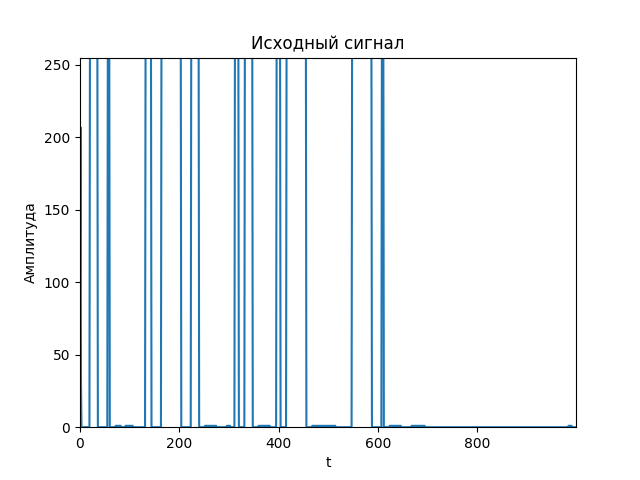
\includegraphics[width=0.8\textwidth]{media/ict/image64}
	\caption*{Рис.1 - Исходный аудиосигнал}
\end{figure}

\begin{figure}[H]
	\centering
	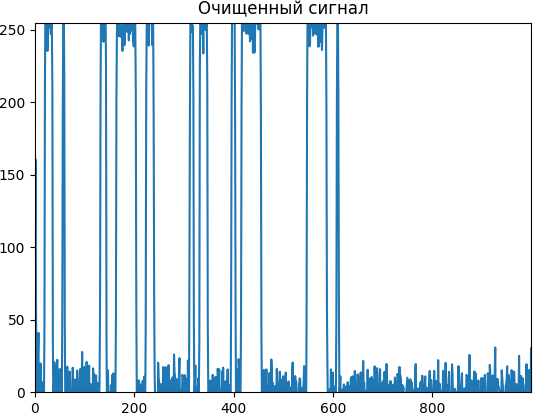
\includegraphics[width=0.8\textwidth]{media/ict/image65}
	\caption*{Рис.2 - Очищенный аудиосигнал}
\end{figure}

\begin{figure}[H]
	\centering
	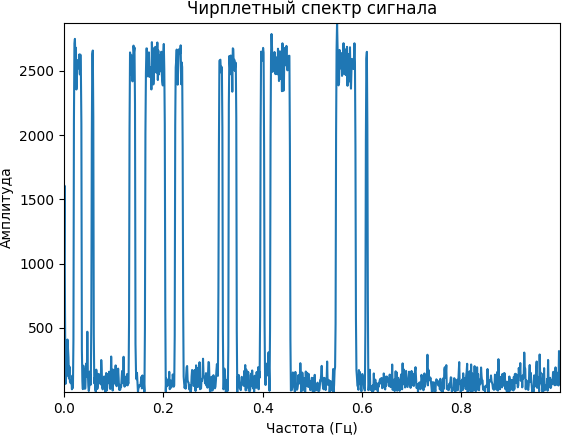
\includegraphics[width=0.8\textwidth]{media/ict/image66}
	\caption*{Рис.3 - Чирплетный аудиосигнал}
\end{figure}

\begin{figure}[H]
	\centering
	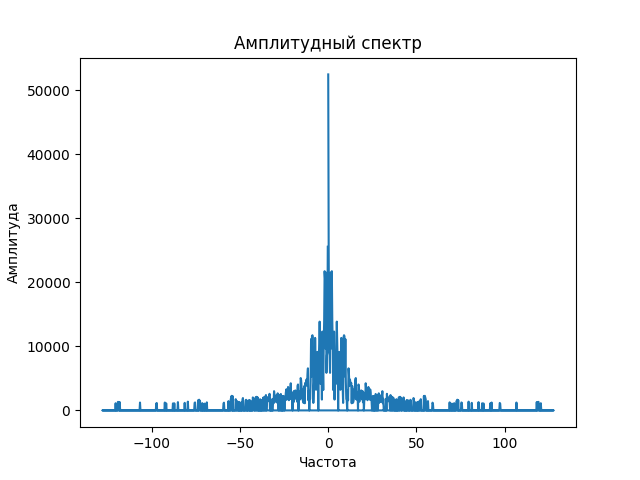
\includegraphics[width=0.8\textwidth]{media/ict/image67}
	\caption*{Рис.4 - Амплитудный спектр чирплетного аудиосигнала}
\end{figure}

\begin{figure}[H]
	\centering
	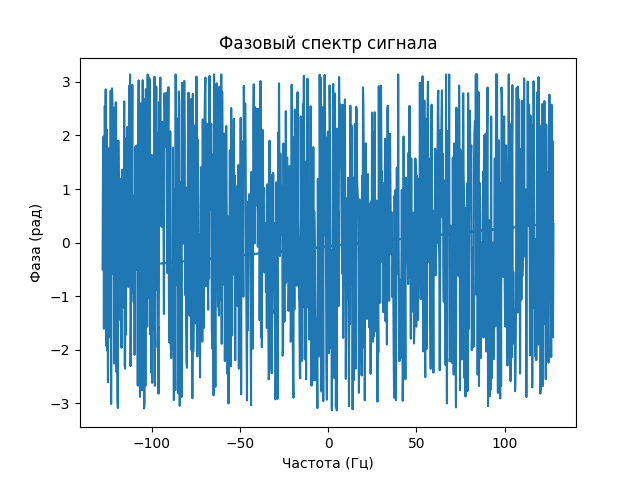
\includegraphics[width=0.8\textwidth]{media/ict/image68}
	\caption*{Рис.5 - Фазовый спектр чирплетного аудиосигнала}
\end{figure}

\begin{multicols}{2}
В результате обработки экспериментальных данных было вычислено, что
достаточно вычисления трех гармоник (Ka=3). В результате обработки
голосового файла вычисляются 6 характеристик:

1) частотные коэффициенты (основные тоны) --
;

2) амплитудные коэффициенты разложения
.

Для отработки предложенного алгоритма были подготовлены аудиозаписи 50
студентов Международного инженерно-технологического университета г.
Алматы. Каждый студент говорил числа от единицы до десяти на русском
языке. Затем в случайном порядке выбиралась аудиозапись и по нему
определялся его диктор. Также исследовалась аудиозапись такого же
содержания человека, не занесенного в базу данных. Точность
распознавания находится в пределах 73-75\%.

{\bfseries Выводы.} Разработка алгоритмов голосовой идентификации
становится важной задачей в цифровом мире. Внедрение новых методов,
основанных на чирплет-преобразованиях, способствует повышению точности
распознавания речи. Дальнейшие исследования направлены на создание
автоматизированной системы идентификации человека для различных
приложений, включая биометрические системы безопасности.

В данной статье был разработан метод распознавания голоса, основанный на
чирплет-преобразованиях.

Чирплеты представляют собой мощный инструмент в анализе нестационарных
сигналов, объединяя преимущества вейвлетов и чирп-сигналов. Они особенно
полезны в областях, где частотный спектр изменяется во времени.

В дальнейшем, используя предложенный подход, планируется разработка
устройства автоматического допуска человека в определенное помещение на
основе микропроцессорной техники и автономного питания.

\emph{{\bfseries Финансирование.} Работа выполнена за счет средств
грантового финансирования научных исследований на 2023--2025 годы по
проекту AP19678157.}
\end{multicols}

\begin{center}
{\bfseries Литература}
\end{center}

\begin{references}
1. Сергиенко А.Б. Цифровая обработка сигналов. - Санкт-Петербург: Питер,
2002. - 608 с. ISBN 5-318-00666-3

2. Афонский А.А., Дьяконов В.П. Цифровые анализаторы спектра, сигналов и
логики. -- Москва: Солон-Пресс, 2009. - 248 с. ISBN 978-5-91359-049-7

3. Гадзиковский В.И. Цифровая обработка сигналов. - Москва: Солон-Пресс,
2017. - 766 с. ISBN 978-5-91359-117-3

4. Сэломон Д. Сжатие данных, изображений и звука. - Москва: Техносфера,
2004. -368 c. ISBN 978-5-94836-027-Х

5. Марков Ю.В., Боков А.С. Проектирование устройств приема и обработки
сигналов. - Екатеринбург: Изд-во Уральского ун-та, 2015. - 112 с. ISBN
978-5-7996-1497-3

6. Дворкович В.П., Дворкович А.В. Оконные функции для гармонического
анализа сигналов. -- Москва: Техносфера, 2016. - 208 c. ISBN
978-5-94836-432-2

7. Фрик П.Г. Обработка и анализ сигналов и изображений в физических
экспериментах. - Пермь: Пермский ГНИУ, 2023. - 115с. ISBN
978-5-7944-4025-6

8. Тульский И.Н. Повышение эффективности передачи мультимедийной
информации методом чирплет-преобразования //Диссер. канд.техн. наук по
спец.05.13.17 - Теоретические основы информатики, Красноярск, 2012. -
119с

9. Рогозинский Г.Г. Перцепционное сжатие звука с использованием
вейвлетных пакетов //Диссер. канд.техн. наук по спец.05.11.18 - Приборы
и методы преобразования изображений и звука, Санкт-Петербург, 2010. -
118с

10. Брежнев А.В. Разработка методов и средств диагностики психической
напряженности на основе вейвлет-анализа сигнала голоса и нечеткой логики
принятия решений //Авт. диссер. канд.техн. наук по спец.05.13.01 -
Системный анализ, управление и обработка информации, Курск, 2005. - 24
с.

11. M. Aliaskar, T. Mazakov, A. Mazakova, S. Jomartova, T. Shormanov.
Human voice identification based on the detection of fundamental
harmonics // IEEE 7th International Energy Conference
(ENERGYCON)\emph{,} 2022, pp.1-4. DOI
10.1109/ENERGYCON53164.2022.9830471.

12. Шорманов Т.С., Мазакова А.Т., Алиаскар М.С., Бургегулов А.Д.,
Саметова А.А., Исимов Н.Т., Джомартова Ш.А., Мазаков Т.Ж.
Программно-аппаратный комплекс дактилоскопической идентификации человека
// Вестник КазУТБ. - Астана, 2024. - № 4(25). - C.1-7
\href{https://doi.org/10.58805/kazutb.v.4.25-721}{DOI
10.58805/kazutb.v.4.25-721}

13. Шорманов Т.С., Мазакова А.Т., Алиаскар М.С., Джомартова Ш.А., Мазаков
Т.Ж. Применение нейронных сетей для идентификации голоса с учетом
казахского акцента // Вестник КазУТБ. - Астана, 2024. - № 4(25). - C.
60-68/ DOI
\href{https://doi.org/10.58805/kazutb.v.4.25-720}{}
\end{references}

\begin{center}
{\bfseries References}
\end{center}

\begin{references}
1. Sergienko A.B. Cifrovaja obrabotka signalov. - Sankt-Peterburg: Piter,
2002. - 608 s. ISBN 5-318-00666-3. {[}in Russian{]}

2. Afonskij A.A., D' jakonov V.P. Cifrovye analizatory
spektra, signalov i logiki. -- Moskva: Solon-Press, 2009. - 248 s. ISBN
978-5-91359-049-7. {[}in Russian{]}

3. Gadzikovskij V.I. Cifrovaja obrabotka signalov. - Moskva: Solon-Press,
2017. - 766 s. ISBN 978-5-91359-117-3. {[}in Russian{]}

4. Sjelomon D. Szhatie dannyh, izobrazhenij i zvuka. - Moskva:
Tehnosfera, 2004. -368 c. ISBN 978-5-94836-027-H. {[}in Russian{]}

5. Markov Ju.V., Bokov A.S. Proektirovanie ustrojstv priema i obrabotki
signalov. - Ekaterinburg: Izd-vo Ural' skogo un-ta, 2015.
- 112 s. ISBN 978-5-7996-1497-3. {[}in Russian{]}

6. Dvorkovich V.P., Dvorkovich A.V. Okonnye funkcii dlja garmonicheskogo
analiza signalov. -- Moskva: Tehnosfera, 2016. - 208 c. ISBN
978-5-94836-432-2. {[}in Russian{]}

7. Frik P.G. Obrabotka i analiz signalov i izobrazhenij v fizicheskih
jeksperimentah. - Perm': Permskij GNIU, 2023. - 115s.
ISBN 978-5-7944-4025-6. {[}in Russian{]}

8. Tul' skij I.N. Povyshenie jeffektivnosti peredachi
mul' timedijnoj informacii metodom
chirplet-preobrazovanija //Disser. kand.tehn. nauk po spec.05.13.17 -
Teoreticheskie osnovy informatiki, Krasnojarsk, 2012. -- 119 s. {[}in
Russian{]}

9. Rogozinskij G.G. Percepcionnoe szhatie zvuka s
ispol' zovaniem vejvletnyh paketov //Disser. kand.tehn.
nauk po spec.05.11.18 - Pribory i metody preobrazovanija izobrazhenij i
zvuka, Sankt-Peterburg, 2010. -- 118 s. {[}in Russian{]}

10. Brezhnev A.V. Razrabotka metodov i sredstv diagnostiki psihicheskoj
naprjazhennosti na osnove vejvlet-analiza signala golosa i nechetkoj
logiki prinjatija reshenij //Avt. disser. kand.tehn. nauk po spec.
05.13.01 - Sistemnyj analiz, upravlenie i obrabotka. {[}in Russian{]}

11. M. Aliaskar, T. Mazakov, A. Mazakova, S. Jomartova, T. Shormanov.
Human voice identification based on the detection of fundamental
harmonics // IEEE 7th International Energy Conference
(ENERGYCON)\emph{,} 2022, pp.1-4. DOI
10.1109/ENERGYCON53164.2022.9830471.

12. Шорманов Т.С., Мазакова А.Т., Алиаскар М.С., Бургегулов А.Д.,
Саметова А.А., Исимов Н.Т., Джомартова Ш.А., Мазаков Т.Ж.
Программно-аппаратный комплекс дактилоскопической идентификации человека
// Вестник КазУТБ. - Астана, 2024. - № 4(25). - C.1-7
\href{https://doi.org/10.58805/kazutb.v.4.25-721}{DOI
10.58805/kazutb.v.4.25-721}. {[}in Russian{]}

13. Шорманов Т.С., Мазакова А.Т., Алиаскар М.С., Джомартова Ш.А., Мазаков
Т.Ж. Применение нейронных сетей для идентификации голоса с учетом
казахского акцента // Вестник КазУТБ. - Астана, 2024. - № 4(25). - C.
60-68. DOI

{[}in Russian{]}
\end{references}

\begin{authorinfo}
\emph{{\bfseries Сведения об авторах}}

Әлиасқар М.С. -- старший преподаватель МИТУ, Алматы, Казахстан, e-mail:

ORCID:
https://orcid.org/\href{https://orcid.org/0000-0002-3013-6617}{}

Джомартова Ш.А. -- доктор технических наук, доцент, КазНУ им.
аль-Фараби, Алматы, Казахстан, e-mail:
jomartova@mail.ru; ORCID:
\href{https://orcid.org/0000-0002-5882-5588}{}

Мазақова Ә.Т. -- преподаватель КазНУ им.аль-Фараби, Алматы, Казахстан,
e-mail: aigerym97@mail.ru; ORCID:
https://orcid.org/{\bfseries 0000-0003-3019-3352}

Мазаков Т.Ж. -- доктор физико-математических наук, профессор, КазНУ им.
аль-Фараби, Алматы, Казахстан, e-mail:
tmazakov@mail.ru; ORCID:
https://orcid.org/ 0000-0001-9345-5167

Майлыбаева А.Д. -- к.ф.-м.н., доцент кафедры «Информатика» Атырауского
университета имени Х. Досмухамедова, Атырау, Казахстан, e-mail:
a.maylibayeva@asu.edu.kz;
ORCID: 0000-0003-0598-4806

Н.Т. Исимов -- заведующий кафедрой МИТУ, Алматы, Казахстан, e-mail:

ORCID: 0000-0003-4765-7870

Бегалиева К.Б. - PhD, cт.преп. Казахский агротехнический
исследовательский университет имени С. Сейфуллина, e-mail:
kalamkas\_b@mail.ru;
ORCID: 0000-0002-4216-9184

ДосаналиеваА.Т. - старший преподаватель кафедры «Компьютерная инженерия»
Алматинского Технологического Университета, Алматы, Казахстан, e-mail:
Dosanalieva1985@gmail.com;
ORCID:0009-0000-2958-1935

\emph{Information about the authors}

Aliaskar M.S. -- Lecturer at the International University of Engineering
and Technology, Almaty, Kazakhstan, e-mail:


Jomartova Sh.A. - Doctor of Technical Sciences, Associate Professor,
Al-Farabi Kazakh National University, Almaty, Kazakhstan, e-mail:
jomartova@mail.ru;

Mazakova A.T.-Lecturer at the Al-Farabi Kazakh National University,
Almaty, Kazakhstan, e-mail:
aigerym97@mail.ru;

Mazakov T.Zh. -- Doctor of Physical and mathematical sciences, professor
Al-Farabi Kazakh National University, professor at the International
University of Engineering and Technology Almaty, Kazakhstan, e-mail:
tmazakov@mail.ru;

Mailybayeva A.D. -- PhD, Associate Professor, Department of Computer
Science, Atyrau University named after Kh. Dosmukhambetov, Atyrau,
Kazakhstan, e-mail:
a.maylibayeva@asu.edu.kz;

Issimov N.T. -- Head of Department at the International University of
Engineering and Technology, Almaty, Kazakhstan, e-mail:


Begaliyeva K.B. -- PhD, Senior Lecturer, Kazakh Agrotechnical Research
University named after S. Seifullin, Astana, Kazakhstan, e-mail:
kalamkas\_b@mail.ru

Dosanalieva A.T. - Senor Lecturer, Computer Engineering Department,
Almaty Technological University, Almaty, Kazakhstan, e-mail:
Dosanalieva1985@gmail.com;
ORCID:0009-0000-2958-1935\
\end{authorinfo}
